% \section{数学工具}
% \subsection{拉普拉斯分布}
% % 合成图像数据集往往假设低分辨率图像由高分辨率图像经高斯模糊和双三次下采样得到,使用公式表示即为:
% % \begin{equation}
% %     \mathbi{I}^{LR}=(\vb*{k}_g\otimes \mathbi{I}^{HR})\downarrow_s
% % \end{equation}
% 拉普拉斯分布是以法国数学家Pierre-Simon命名的一种连续概率分布,又称双指数分布。拉普拉斯分布的概率密度函数为
% \begin{equation}
%     f(x;\mu, b)=\frac{1}{2b}\exp(-\frac{|x-\mu|}{b})
% \end{equation}
% 其中,$\mu$为位置参数,表示其对称轴位置;$b$为尺度参数,表示其开口尺度。其概率密度函数与累计分布函数如图\ref{fig:laplace-a}\ref{fig:laplace-b}所示。在本文所基于的模型USR-DU中,作者经过实验发现真实的低分辨率图像与双三次下采样图像之间的差异呈拉普拉斯分布,如图\ref{fig:laplace-c}所示。
% \begin{figure}[h]
%     \subcaptionbox{\label{fig:laplace-a}}{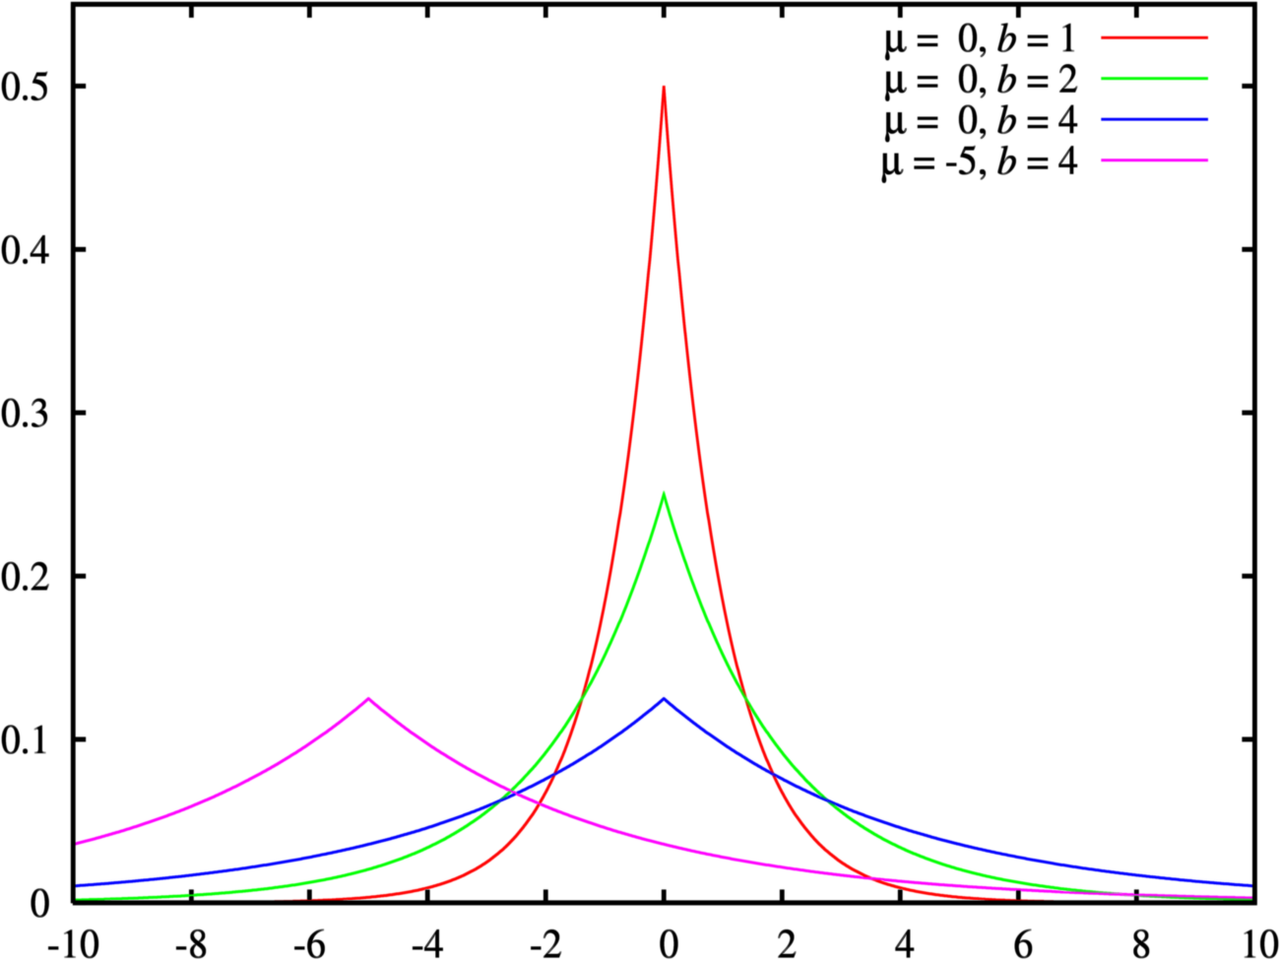
\includegraphics[width=.3\linewidth]{imgs/laplace_wiki_1.png}}\hfill
%     \subcaptionbox{\label{fig:laplace-b}}{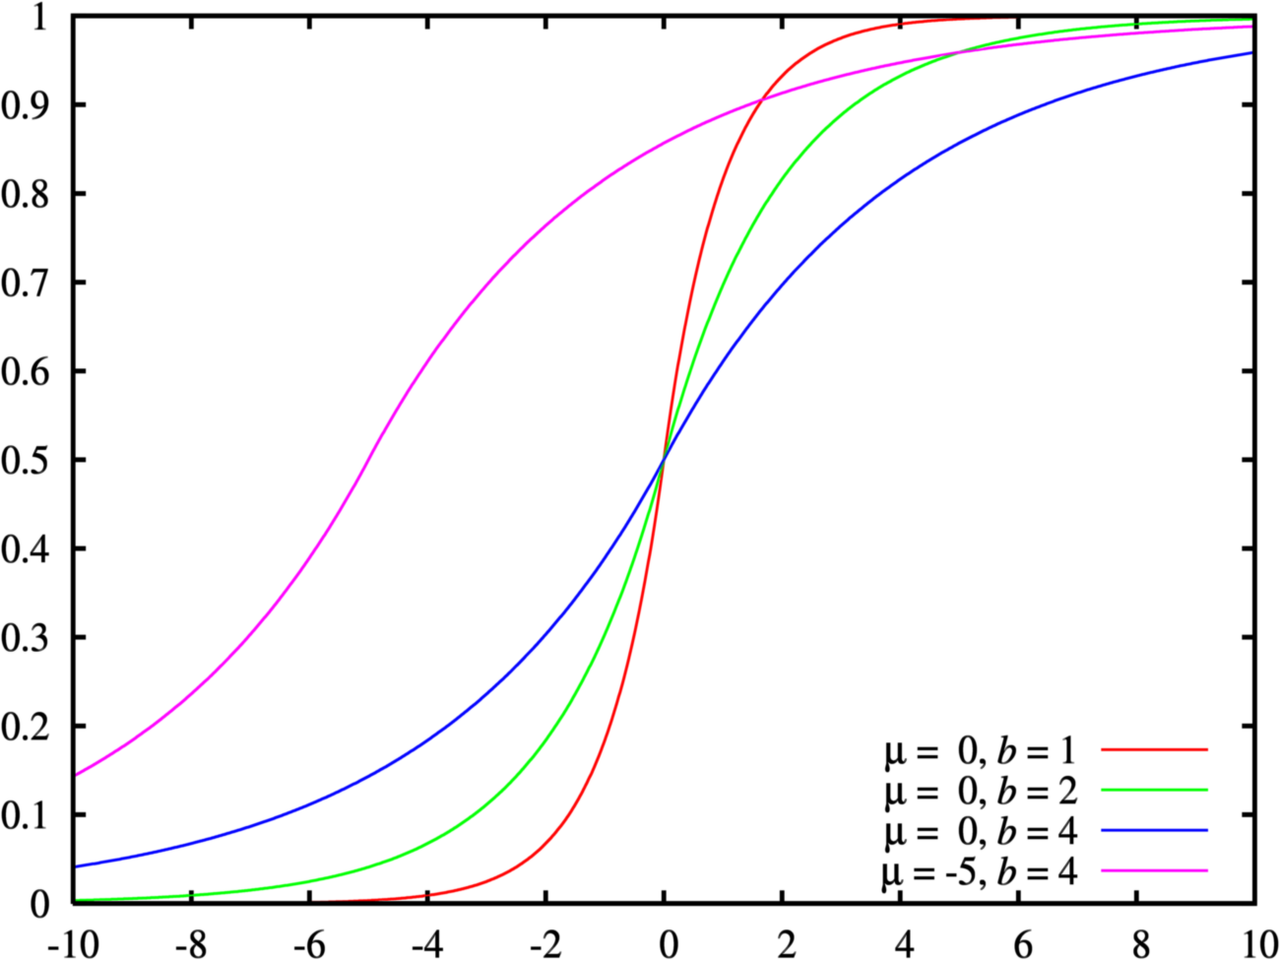
\includegraphics[width=.3\linewidth]{imgs/laplace_wiki_2.png}}\hfill
%     \subcaptionbox{\label{fig:laplace-c}}{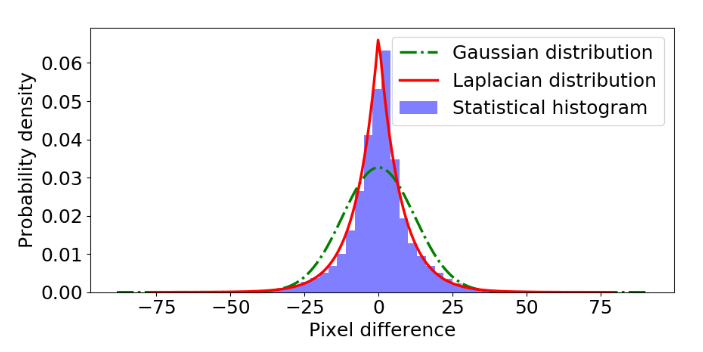
\includegraphics[width=.4\linewidth]{imgs/laplace_usr-du.png}}
%     \caption{拉普拉斯分布:其中,图(a)为概率密度函数,图(b)为累计分布函数,图(c)为USR-DU论文中作者对真实低分辨率图像与双三次下采样图像间差异分布进行实验的结果,作者发现实际的分布近似于拉普拉斯分布而不近似于高斯分布}	
%     \label{fig:laplace}
% \end{figure}

% \subsection{KL散度}
% KL散度(Kullback-Leibler divergence)又称相对熵,描述了$P$,$Q$两个分布之间的差异,其中$P$为真实分布,$Q$为估计分布。对于连续随机变量,KL散度可定义为
% \begin{equation}
%     D_{\text{KL}}(P\|Q)=\int^\infty_{-\infty}p(x)\ln\frac{p(x)}{q(x)}\,\text{d}x
% \end{equation}

% 在USR-DU中,DSN输出低分辨率图像$\vb*{y}_g$及其不确定性$\bm{\theta}$,其实质为输出了估计的低分辨率图像的分布。故为了优化网络,使其估计出正确的分布,可使用KL散度来构造损失函数
% \begin{equation}
%     \begin{aligned}
%         \mathcal{L}_{kl}&=\mathbb{E}_{\vb*{y}_g}\{D_{\text{KL}}[L(\vb*{y}_g,\bm{\theta})\|L(\vb*{y}_b,\mathbi{I})]\}  \\
%         &=\mathbb{E}_{\vb*{y}_g}[\bm{\theta}\exp(-\frac{\|\vb*{y}_g-\vb*{y}_b\|_1}{\bm{\theta}})+\|\vb*{y}_g-\vb*{y}_b\|_1-\ln\bm{\theta}-1]
%     \end{aligned}
%     \label{equ:kl}
% \end{equation}
% 其中$\vb*{y}_b$为双三次下采样图像,$\mathbi{I}$为单位矩阵。


\section{超分辨率模型的评价指标}
为了能够评判各种超分辨率模型间精度的优劣,需要采用多种指标进行评价。而不同的评价指标则拥有不同的侧重点。
\subsection{基于参考的评价指标}
此类指标是最常用的评价指标。其中,PSNR(Peak Signal-to-Noise Ratio,峰值信噪比)通过比较原始图像与经过处理后的图像的信噪比来衡量两张图像之间的差距,单位为分贝(dB),取值范围为0到无穷大。PSNR越大,则说明两张图像越相近。PSNR的定义式为:
\begin{equation}
    \text{PSNR}=10\cdot \log_{10}(\frac{\text{MAX}_I^2}{\text{MSE}})
\end{equation}
其中,$MAX_I$是像素的最大值,这取决于像素值是$0\sim 255$还是$0\sim 1$;MSE(Mean Square Erros)是两张图像之间的均方误差。

SSIM\parencite{wang2002universal}(Structural Similarity Index Measure,结构相似性指标)除了考虑除了像PSNR考虑像素间差异以外,还考虑图像的结构、纹理、对比度等因素。SSIM没有单位,取值范围为-1到1,SSIM越大,说明两张图像相似度越高。SSIM的定义为
\begin{equation}
    \begin{aligned}
        SSIM(x,y)&=[l(x,y)s(x,y)c(x,y)]
                 &=\frac{(2\mu_x\mu_y+c_1)(2\sigma_{xy}+c_2)}{(\mu_x^2\mu_y^2+c_1)(\sigma_x^2+\sigma_y^2+c_2)}
    \end{aligned}
\end{equation}
其中,$l(x,y)$代表亮度,$s(x,y)$代表结构,$c(x,y)$代表对比度。$\mu_x$、$\mu_y$代表$x、y$的均值,$\sigma_x$、$\sigma_y$代表$x、y$的方差,$\sigma_{xy}$代表$x、y$的协方差,$c_1$、$c_2$为常数。实际计算中,采用滑动窗口法,即计算图像中每一个窗口的SSIM,最后取其平均值。

\subsection{基于感知的评价指标}
以上两种评价指标基本侧重于图像的像素和结构,二者的计算较为机械,有时候PSNR和SSIM指标高的图像并不能很好地满足人类的需求,故某些工作招募志愿者用肉眼对图像进行打分,但是这种评判方式具有较大的主观性,因此需要一个能够定量评判感知质量的评价指标。而LPIPS\parencite{zhang2018perceptual}(Learned Perceptual Image Patch Similarity,学习的图像像素相似性指标)就是其中具有代表性的一个指标。此指标通过卷积神经网络来学习人类对图像的感知差异。从计算方式上来说,此指标通过计算两张图像通过预训练的卷积神经网络提取得到的特征图之间的余弦距离来评判图像间的相似性,指标越接近于0,则说明两张图像在人类感知上越相近。由于侧重点不同,有时会出现LPIPS指标很优而PSNR/SSIM很劣或者PSNR/SSIM很优LPIPS很劣的情况,这个时候就要结合需求综合分析模型的优劣。

\section{合成图像超分辨率技术}
早期,许多超分辨率模型通常假设高分辨率图像是通过高斯模糊和双三次下采样退化为低分辨率图像的,其训练集与测试集都是采用上述退化过程产生的合成数据集。我们称这些方法为合成图像的超分辨率技术。
\subsection{传统的图像超分辨率技术}
在2014年以前,图像超分辨率技术主要采用计算机视觉领域中传统的方法。其中包括插值、稀疏表示、局部嵌入等,其中最基础的方法是基于插值算法的上采样。常用的插值算法可分为双线性插值、双二次插值和双三次插值,其精细度依次增加。由于超分辨率是使图像的像素增加的过程,这意味着原图中的像素之间将会加入更多像素。由于图像的像素是离散的,而我们并不知道真实的描述图像的连续函数$f(x,y)$,故为了确定新增像素的值,可以使用插值算法,即给出一个插值函数$g(x,y)$,其中对于图像中的每个像素$f(x_i,y_i)$,有$g(x_i,y_i)=f(x_i,y_i)$。对于新增的像素点,使用插值函数算出其值即可。插值算法的优点是简单、快速,缺点是不够真实,不能补充较为详细的细节信息。

随着技术的发展,稀疏表示方法逐渐成为研究的热点。Yang等人\parencite{4587647}指出,可将图像分解为字典$D$与原子$\alpha$,其中高、低分辨率图像的原子类似,而字典不同。此算法首先使用成对的高低分辨率数据集训练字典,在推理时,通过字典$D_l$计算出低分辨率图像的原子,再使用此原子与高分辨率图像的字典$D_h$计算出高分辨率图像。由于最初的稀疏表示方法没有考虑图像的噪声、模糊的问题,Dong等人\parencite{6392274}提出了稀疏编码噪声的概念,将算法优化目标转为降低稀疏编码噪声,通过图像非局部自相似性获得了对图像稀疏编码的良好估计。稀疏编码方法在PSNR与SSIM\parencite{wang2002universal}指标上较插值算法更高,也能还原更多的细节,但生成的高分辨率图像中带有较为明显的锯齿。


\subsection{基于卷积神经网络的超分辨率技术}
随着AlexNet\parencite{NIPS2012_c399862d}在2012年的ImageNet竞赛中得冠,基于深度卷积神经网络的模型逐渐进入计算机视觉研究者的视野,而后续的VGG\parencite{simonyan2014very}、GoogleNet\parencite{szegedy2015going}等则更让此类方法成为了计算机视觉研究的主流。2014年,Dong等人\parencite{SRCNN}提出了基于卷积神经网络的SRCNN,开创了使用深度学习方法研究图像超分辨率问题的先河。作者将传统稀疏表示方法的过程抽象为三层卷积神经网络,其中第一层提取低分辨率图像的特征图,第二层将特征图与高分辨率图像的稀疏表示相对应,第三层结合空间邻域的预测完成高分辨率图像的重建。SRCNN在保证其推理速度更快的同时,其超分辨率效果远超其他传统模型。

\subsubsection{典型超分辨率模型的结构}
卷积神经网络是一种由卷积层、池化层、全连接层等模块组成的一种人工神经网络。其中,卷积层会使用多个卷积核对输入张量进行卷积操作,并输出通道数等于卷积核数量的特征图,特别的,对于$1\times 1$卷积,相当于在每个像素的通道维度上做全连接;池化层会通过某种方式(如最大值、平均值)等对输入张量进行下采样,缩小输入的维度;而全连接层则为多层感知机(MLP)网络,对输入张量进行全连接,最后的输出向量可用于分类、回归等任务。在图像超分辨率这一领域中,卷积神经网络中一般不使用全连接层,而是直接输出一张结果图像。如图\ref{fig:SRCNN}是SRCNN模型的结构,输入图像首先双三次上采样到期望的尺寸,然后经过一个卷积核尺寸$9\times 9$,拥有64个卷积核的卷积层,输出一个64通道的特征图;再经过一个卷积核尺寸$1\times 1$,拥有32个卷积核的卷积层,输出一个32通道的特征图;最后经过一个卷积核尺寸$5\times 5$,拥有3个卷积核的卷积层,输出一个3通道的特征图,而此输出则为最终生成的高分辨率图像。
\subsubsection{典型超分辨率模型的训练和推理}
对于简单的卷积神经网络如SRCNN,可以使用监督式训练。训练过程中,输入batch中会包含成对的高分辨率和低分辨率图像。网络输入低分辨率图像,输出超分图像,用超分图像和高分辨率图像计算均方差损失函数(MSE Loss),随后使用随机梯度下降(SGD)等优化器对模型参数进行优化,经过若干次迭代,直到损失函数收敛。在推理时,只需要输入低分辨率图像,即可使用训练好的模型生成超分图像。

\begin{figure}[h]
    \centering
    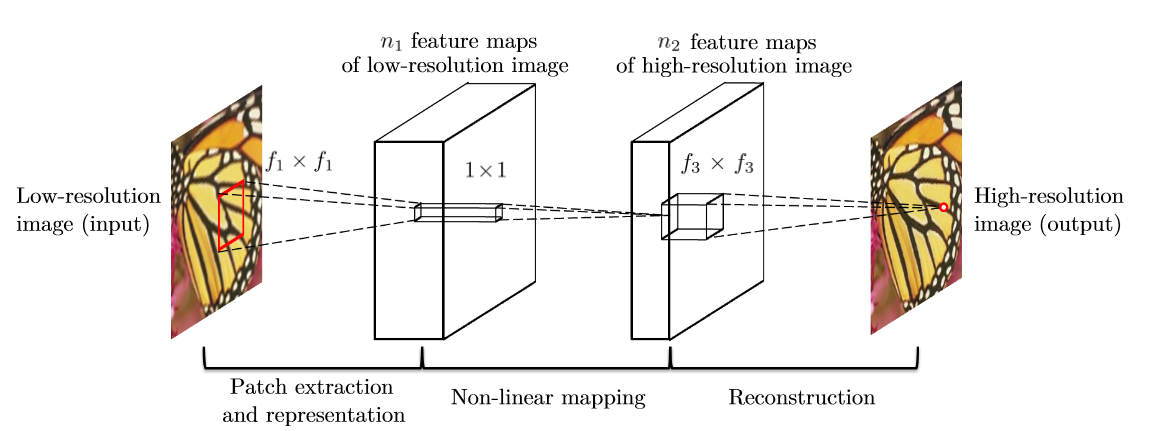
\includegraphics[width=1.0\textwidth]{imgs/SRCNN.png}
    \caption{SRCNN的结构}
    \label{fig:SRCNN}
\end{figure}

\subsubsection{基于卷积神经网络的超分辨率技术的发展}
由于SRCNN只有三层,其并没有完全利用深度卷积神经网络的优势。在接下来一段时间中,研究者提出了多种改进模型,从模型深度、残差连接、密集(dense)连接等角度对基于卷积神经网络的超分辨率模型进行了优化,使模型在准确度方面有了进一步的提升。但对于较大的放大倍数,这些模型却无法恢复出较为精细的纹理细节。随着生成对抗网络\parencite{goodfellow2020generative}(GAN)这一框架在计算机视觉领域中逐渐流行,Ledig等人\parencite{fritsche2019frequency}提出了基于GAN的模型SRGAN,其中,生成器负责生成更为真实的高分辨率图像,而判别器则负责分辨生成的高分辨率图像和真实数据集中的高分辨率图像。通过这一框架,对大的放大倍率来说,可以重建出更逼真的图像。此后,超分辨率模型多会基于GAN设计,本文亦是如此。

\section{真实图像超分辨率技术}
当将合成图像超分辨率模型应用于真实场景下时,会发现图像的重建能力严重下降,并产生难以预料的伪影。这是由于真实高分辨率图像是通过噪声、模糊、图像压缩等未知且复杂的方式退化为低分辨率图像,导致真实的低分辨率图像与合成的低分辨率图像在纹理细节、模糊程度等方面完全不一致。

为了解决真实图像的超分辨率问题,可以使用真实成对的数据集(如City100\parencite{chen2019camera},RealSR\parencite{cai2019toward}等)训练超分辨率网络,从而提升模型对真实图像的重建能力。但是,从一方面来说,真实成对数据集的采集工作是费时费力且高成本的,故无法取得大量的;从另一方面来说,对于某些任务来说(如修复老照片,老电影等),低分辨率图像本身没有对应的高分辨率图像,无法进行监督式的训练。因此,必须对模型本身进行改进,以满足真实图像超分辨率任务的需求。在发展早期阶段,Yuan等人\parencite{yuan2018unsupervised}提出了无监督模型CinCGAN,作者利用两个CycleGAN\parencite{zhu2017unpaired},分别将低分辨率图像进行去模糊去噪处理和超分辨率,其中生成性损失通过重构损失和内容损失(identity loss)计算,第一个网络使用干净的非成对的低分辨率图像计算对抗性损失,而第二个网络使用非成对的高分辨率图像计算对抗性损失。作为无监督模型,CinCGAN取得了和监督式模型相当的超分辨率效果,但由于模型过于复杂,带来了许多精度上的下降。

为了能以较小的计算成本去训练一个更具泛化性的模型,Fritsche等人\parencite{fritsche2019frequency}开创性地提出了DSGAN模型,意为DownSampleGAN。该模型由两部分组成,依次进行训练。其中,第一部分为下采样模型,将高分辨率图像退化为贴近真实的低分辨率图像。为保证这一点,使用高频滤波获得生成图像与真实图像的高频信息(纹理细节),并计算对抗损失。通过此模型,可以针对只有高分辨率图像的数据集生成大量伪成对的低分辨率图像。而第二部分为超分辨率模型,使用第一部分模型生成的伪成对数据集进行训练。基于这一模型框架,许多后续工作在生成图像与真实图像的域差距、显式估计模糊核、退化的随机性等方面优化了这一框架的性能。然而,这些工作往往假定图像的退化过程是确定性的,即一张高分辨率图像只能退化为一张低分辨率图像。而实际情景中,由于各种因素影响,图像的退化过程往往是具有不确定性的,即一张高分辨率图像可以经由不同的方式退化为不同的低分辨率图像。

为了估计这种不确定性,并将其用于更好地生成低分辨率图像,Ning等人\parencite{ijcai2022p176}提出基于不确定性学习的无监督超分辨率模型USR-DU。作者首先探究了真实图像的退化规律,发现真实的低分辨率图像与双三次下采样图像之间的差异可以使用拉普拉斯分布来表征,该分布的位置参数代表了低分辨率图像的基准像素值,而尺度参数则代表了像素值的不确定性。与上述工作类似,此模型分为降采样部分DSN和超分部分SRN。其中,DSN输入高分辨率图像,生成拟真的低分辨率图像及其不确定性,二者拥有相同的尺寸。生成的低分辨率图像与高分辨率图像的双三次下采样结果计算内容损失,与非成对的真实低分辨率图像计算对抗性损失。为了确保生成图像及其不确定性也满足拉普拉斯分布,在计算内容损失时,采用KL散度使得生成的分布逼近实际的分布。为了能在特征域也考虑不确定性,DSN另外生成了拟真低分辨率图像经由VGG提取的特征图的不确定性,并使用生成图像的特征图与双三次下采样图像的特征图计算感知损失(同样使用KL散度)。在DSN网络训练完成后,使用DSN生成大量的伪成对数据集训练SRN。其中,伪成对数据集中的低分辨率图像由生成的低分辨率图像及其不确定性依照拉普拉斯分布随机采样获取。借由不确定性学习,USR-DU在减少伪影的同时提高了超分辨率图像的清晰度。但是,当将此模型应用到模型性较大的数据集(如RealSR)中时,其超分辨率性能有所下降。这是由于其DSN部分忽略了图像退化过程中的模糊性因素,直接使用了干净的双三次下采样图像作为参考图像,而如何在DSN中引入模糊信息,则是本文研究的重点。

\section{基于模糊核估计的盲图像超分辨率技术}
除了上述方法,也有部分工作采取显式估计模糊核,并将模糊核作为特征融合到超分辨率网络中的方式来训练真实图像超分辨率模型。其中,Liang等人\parencite{liang2021mutual}提出了MANet,训练了一个空间变化地估计低分辨率图像模糊核的网络,并使用此网络对修改过的RRDB-SFT超分网络进行微调,从而实现真实图像超分辨率。Fang等人\parencite{fang2022uncertainty}提出了KULNet,同步训练了核估计网络和超分辨率网络,并引入了不确定性学习,增强了模型的稳定性。Fang等人\parencite{fangself}提出了UFPNet,基于流模型空间可变地估计了运动模糊核,具体来说,首先训练了一个可生成运动模糊核的流模型,再训练了一个模糊核隐代码估计网络,使用估计的隐代码来生成最终的模糊核,其中,隐代码的估计采用了不确定性学习。随后,将估计的模糊核融合到超分辨率网络中。此模型兼顾了空间可变模糊核估计和不确定性学习,使得模型的稳定性和准确性进一步增强。本文中,为了解决如何在USR-DU的降采样部分中引入模糊信息的问题,对上述核估计模型的利用必不可少。

